% =========================================================================== %

\begin{frame}[t,plain]
\titlepage
\end{frame}

% =========================================================================== %

\begin{frame}{Programmieren in C und C++ -- Einsteigerkurs}
% C++ -- hardly at all
% this is introduction.
% possibly some sites where to look up commands
% Kurs-Schlüssel in PPT?
%
\begin{columns}[T]
\column{.7\linewidth}
\begin{itemize}
\item C: Sprache für hochoptimierte (effiziente) Lösungen
	\begin{itemize}
	\item Treiber für Gerätesteuerung
	\item Numerische Lösungen
	\item Betriebssystem-Kernels (\zB Linux!)
	\end{itemize}
\item Hier: Erste Schritte, kleinere Projekte
\item Konzepte auf (fast) alle Programmiersprachen übertragbar
\item C++: Eigenständige Sprache; hier nur als Ausblick
	\begin{itemize}
	\item alle Konzepte aus C
	\item Neue Strukturen, komplexere Programme übersichtlicher
	\item \enquote{Paradigma} Objektorientierung
	\end{itemize}
\end{itemize}
\column{.3\linewidth}

\includegraphics[width=\linewidth]{./gfx/T-Pudel-C}\newline
\tiny Danke, Lea.
\end{columns}
%
\end{frame}

% =========================================================================== %

\begin{frame}
%
\begin{minipage}[T]{.49\linewidth}
\begin{Large}
{Grundbegriffe: Compiler}
\end{Large}
\begin{itemize}
\item Mensch und Maschine \enquote{denken} unterschiedlich
\item Mehrere Stufen der Übersetzung nötig
\item Mensch: komplexe Konstrukte (\emph{schreibe in eine Datei})
\item Maschine: sehr einfache Teilschritte (\emph{addiere Zahlen})
\item Maschine: Ultimativ nur Zahlen; numerierte Anweisungen
\item Compiler: Erledigt letzte Übersetzungsschritte von Code für Menschen zu Code für Maschinen
\end{itemize}
\end{minipage}
%
\begin{minipage}{.49\linewidth}
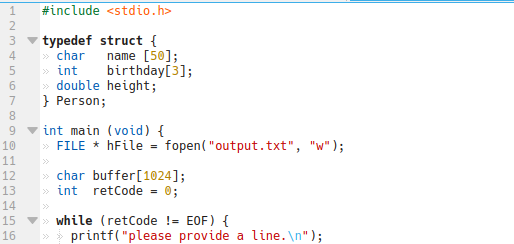
\includegraphics[width=\linewidth]{./gfx/CodeRaw}
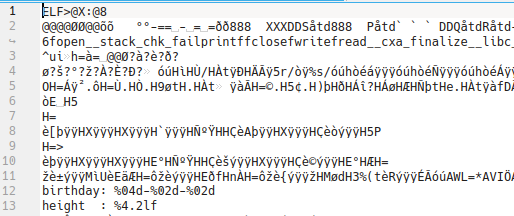
\includegraphics[width=\linewidth]{./gfx/CodeCompiled}
\end{minipage}
%
\end{frame}

% =========================================================================== %

\begin{frame}[fragile]{Objekte Arbeitsspeicher}
%
\begin{columns}
\column{.5\linewidth}
	\begin{itemize}
	\item \emph{Alle} Objekte letztlich nur Zahlen
	\item Beispiel Buchstaben: Zuordnung \newline 
		Zahlen $\leftrightarrow$ Glyphen durch Tabelle
	\item Komplexere Elemente: Gruppe von Zahlen
	\item Beispiel Bild: Rot-, Grün-, Blauanteil erster Pixel, zweiter Pixel, \ldots
	\item Lediglich der Kontext gibt vor, wie Daten interpretiert werden sollen!
	\end{itemize}
\column{.5\linewidth}
	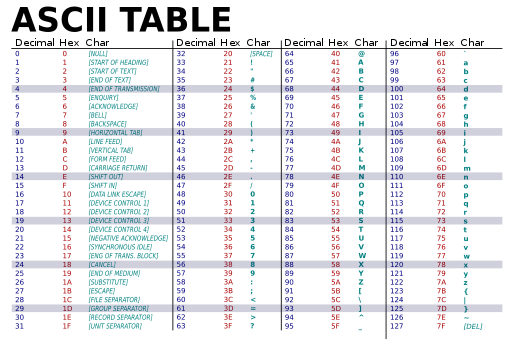
\includegraphics[width=\linewidth]{./gfx/ASCII_table}\newline
	\tiny ASCII: American Standard Code for Information Interchange\newline
	Quelle: \url{source: https://commons.wikimedia.org/wiki/File:ASCII-Table-wide.svg}
\end{columns}
%
\end{frame}

% =========================================================================== %

\begin{frame}[fragile]{Modell eines Computers}
%
\begin{columns}
\column{.4\linewidth}
\begin{itemize}
\item Maschinensprache: Bytecode (\enquote{nummerierte Befehle})
\item Sehr simple Anweisungen
\item \enquote{Legen Schalter im Prozessor um}
	\begin{itemize}
	\item Register: Kleine Speicherzellen im Prozessor. Fassen wenige Byte. 
	\item Hier werden Berechnungen umgesetzt.
	\end{itemize}
\end{itemize}
%
\column{.7\linewidth}
\begin{adjustbox}{max totalsize={.9\textwidth}{.7\textheight},center}
\begin{tikzpicture}
  [ 
    cell/.style={text width=8mm,
      text height=4mm, draw=black, inner sep=1mm},
    ld/.style={draw=blue,shorten >=2pt,->}
  ]
  \node (load1) at ( 0,0) [cell] {\scriptsize\ttfamily load};
  \node (adr1)  at ( 1,0) [cell] {\scriptsize\ttfamily 538};
  \node (load2) at ( 2,0) [cell] {\scriptsize\ttfamily load};
  \node (adr2)  at ( 3,0) [cell] {\scriptsize\ttfamily 537};
  \node (add)   at ( 4,0) [cell] {\scriptsize\ttfamily add};
  \node (store) at ( 5,0) [cell] {st};
  \node (adr3)  at ( 6,0) [cell] {\scriptsize\ttfamily 537};
  \node (num2)  at ( 7,0)        {\scriptsize\ttfamily \ldots};
  \node (num1)  at ( 8,0) [cell] {23};
  \node (num2)  at ( 9,0) [cell] {42};
  \node [right=1cm of num2] {Speicher};
    
  \node (nload1) [color=red,above=2mm of load1] {71};
  \node (nload2) [above=2mm of load2]           {73};
  \node (nadd)   [above=2mm of add]             {75};
  \node (nst)    [above=2mm of store]           {76};
  \node (nnum1) [above=2mm of num1]             {537};
  \node (nnum2) [above=2mm of num2]             {538};

  \draw [fill=white!80!black]  (3,-3) rectangle (7,-6);
  \node [anchor=south east] at (7,-6) {Prozessor (CPU)};
  \node [cell,fill=white] (r1)  at  (3.5,-3.5) {reg.};
  \node [cell,fill=white] (r2)  at  (3.5,-4.5) {reg.};
  \node [cell,fill=white] (dec) at  (3.5,-5.5) {dec.};
  \node [cell,fill=white] (ip)  at  (5.0,-3.3) {IP};

  \node [coordinate,left=1cm of load1] (help) {};

  \draw [ld] (load1.south) .. controls +(0,-1) and +(-1,0) ..  (dec.west);
  \draw [draw=red] (nload1) .. controls +(-.5,0) and +(0,.5) .. (help);
  \draw [draw=red] (help) .. controls +(0,-2) and +(0,2) .. (ip);
  \draw [ld,draw=orange] (num2) ..controls +(0,-2) and +(-5,2) .. (r1);
\end{tikzpicture}
\end{adjustbox}
\end{columns}
%
\end{frame}

% =========================================================================== %

\begin{frame}[fragile]{Arbeitsschritte des Kompilers}
%
\begin{columns}
\column{.4\linewidth}
\begin{itemize}
\item Kompilieren
	\begin{itemize}
	\item Übersetzen in Assembler (beinahe Maschinensprache)
	\end{itemize}
\item Assemblieren
	\begin{itemize}
	\item Übersetzen Maschinensprache (Object-Files)
	\end{itemize}
\item Linken
	\begin{itemize}
	\item Verknüpfen zu einer einzigen Ausführbaren Datei
	\item Eigene Object-Files
	\item Vorkompilierte Libraries (Routinen-Sammlungen)
	\end{itemize}
\end{itemize}
%
\column{.6\linewidth}
\begin{adjustbox}{max totalsize={.9\textwidth}{.7\textheight},center}
\begin{tikzpicture}[
  file/.style={shape=rectangle,draw=black,rounded corners=2pt},
  tool/.style={shape=ellipse,draw=black},
  flow/.style={draw=black,->,shorten >=2pt}
]
  \node[file] (programm) {programm.c};
  \node[file, right=1cm of programm] (stdio) {stdio.h};
  \node[file, right=1cm of stdio] (math) {math.h};
  \node[tool, below=2cm of programm] (compiler) {compiler};
  \node[file, below=1cm of compiler] (object) {programm.o};
  \node[file, right=1cm of object] (libm) {libm};
  \node[file, right=1cm of libm] (code) {object code};
  \node[tool, below=1cm of object] (linker) {linker};
  \node[file, below right=2cm and -1cm of linker,text width=4cm] (exe)
    {a.out oder a.exe\\(Ausführbare Datei)};
  \node[coordinate, above left=5mm and 7mm of compiler.north west] (b1) {};
  \node[coordinate, below right=2cm and 5mm of code.south east] (b2) {};
  \draw [blue] (b1) rectangle (b2);
  \node [right=5mm of code, text width=6cm]
  {\color{blue}Meist ein Schritt. Hier oft:\\
  {\small\ttfamily gcc -std=c11 programm.c -lm}};
  \draw[flow] (programm) -- (compiler);
  \draw[flow] (stdio) -- (compiler);
  \draw[flow] (math) -- (compiler);
  \draw[flow] (compiler) -- (object);
  \draw[flow] (object) -- (linker);
  \draw[flow] (libm) -- (linker);
  \draw[flow] (code) -- (linker);
  \draw[flow] (linker) -- (exe);
\end{tikzpicture}
\end{adjustbox}
\end{columns}
%
\end{frame}

% =========================================================================== %

\begin{frame}
%
\begin{columns}[T]
\column{.5\linewidth}
\begin{Large}
{Grundbegriffe: Terminal}
\end{Large}
\begin{itemize}
\item Compiler-Aufruf (wenigstens mittelbar) über ein \emph{Terminal}
\item Mensch-Maschine-Interface
\item Befehle in menschlicher (oder Menschen-ähnlicher) Sprache
\item Bis heute das \emph{Backend}, über das Computer funktionieren.
\item \emph{IDEs} (integrated development environment): mehr Komfort, aber uneinheitlich
\item Letztlich überall Terminal-Kenntnisse nötig, wo Programmiert werden soll
\end{itemize}
%
\column{.5\linewidth}
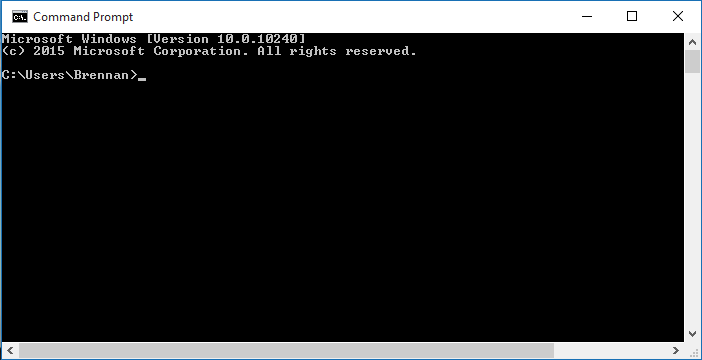
\includegraphics[width=\linewidth]{./gfx/cmd}
{\tiny Windows-Konsole: \texttt{cmd}}
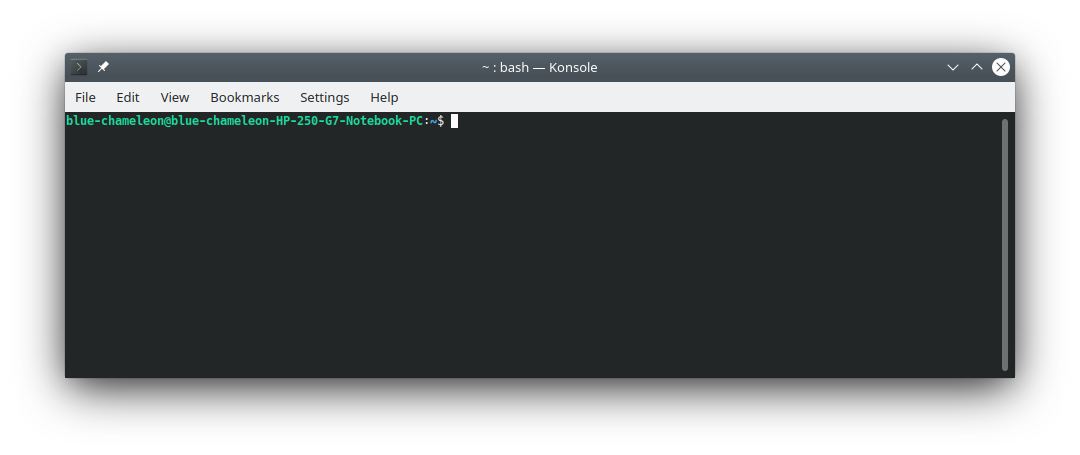
\includegraphics[width=\linewidth]{./gfx/bash}
{\tiny Linux-Konsole: \texttt{bash}}
\end{columns}
%
\end{frame}

% =========================================================================== %

\begin{frame}{Grundbegriffe: Arbeitsverzeichnis}
%
\begin{itemize}
\item Alle Dateien auf Computern: In Ordnern strukturiert
\item Mehrere Dateien mit gleichem Namen in verschiedenen Ordnern möglich
\item Computer muss wissen, welche Datei gemeint ist
\item Idee: Arbeitsverzeichnis: \emph{Wo bin ich gerade}
\end{itemize}
%
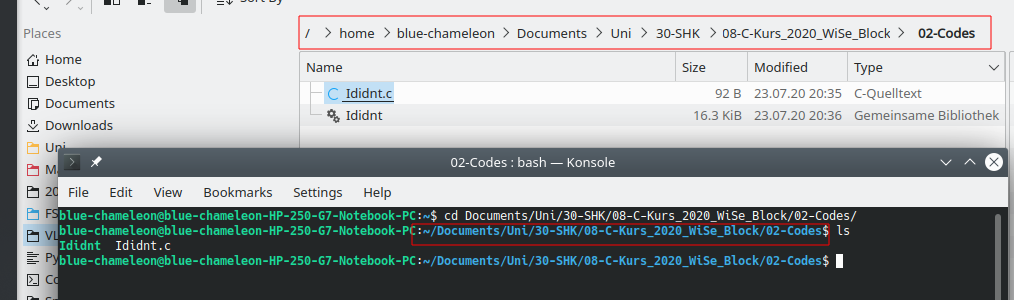
\includegraphics[width=\linewidth]{./gfx/paths}
%
\end{frame}

% =========================================================================== %

\begin{frame}{Programme Starten und Arbeitsverzeichnisse}
%
\begin{itemize}
\item In das richtige Verzeichnis wechseln: \texttt{cd}
	\begin{minipage}{\linewidth}
		\begin{minipage}{.49\linewidth}
		\begin{itemize}
		\item In einem Schritt mehrere Ebenen:\\
			\texttt{cd directory/subdirectory}
		\end{itemize}
		\end{minipage}
		%
		\begin{minipage}{.49\linewidth}
		\begin{itemize}
		\item Oder in mehreren Schritten:\\
			\texttt{cd directory}\\
			\texttt{cd subdirectory}
		\end{itemize}
		\end{minipage}
	\end{minipage}
	\item Eine Ebene zurück: zwei Punkte:\\
		\texttt{cd ..}
	\item Leerzeichen im Pfad? \Thus mit Anführungszeichen einrahmen:\\
		\texttt{cd "Path with whitespaces"}
%	\end{itemize}
\item Name des Programms benennen -- läuft
\end{itemize}
%
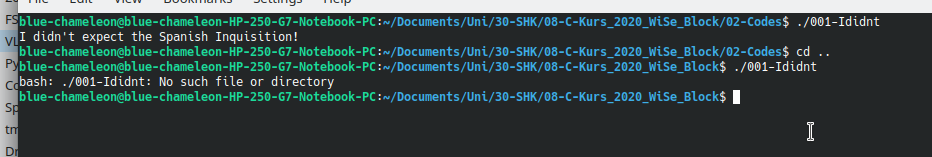
\includegraphics[width=\linewidth]{./gfx/RunRunnot}
%
\end{frame}

% =========================================================================== %

\begin{frame}{Parameter}
%
\begin{itemize}
\item Programme brauchen manchmal zusätzliche Informationen
\item Text hinter dem eigentlichen Befehl
\item Beispiel \texttt{cd}: Unterordner oder \texttt{..}
\item Durch Leerzeichen abgetrennt
\item Auch mehrere Parameter möglich, dann auch jeweils durch Leerzeichen getrennt
\item Problem: Dateinamen mit Leerzeichen
\item Lösung: \texttt{"Text mit Leerzeichen in Anführungszeichen"}
\item Beispiel
	\begin{itemize}
	\item \texttt{notepad ''some file I want to open.txt"}
	\end{itemize}
\end{itemize}
%
\end{frame}

% =========================================================================== %

\begin{frame}{Grundbegriffe: (Dateinamen-)Erweiterung oder Dateiendung}
%
\begin{itemize}
\item Konzept zur Unterscheidung von Datentypen
\item Namenschema \texttt{Inhalt.Typ}
\item Üblicherweise 1-3 Zeichen, seit den späten 90ern aber prinzipiell keine Grenzen
\item txt, pdf, docx, odt, ...
\item Unter Windows häufig ausgeblendet
\item Executables in Windows: \texttt{*.exe}
\item Unixoide Systeme (Linux, Mac OS): meist keine Erweiterungen
\item C-Codes \emph{müssen} aber in allen Betriebssystemen auf \texttt{*.c} (bzw. später auch auf \texttt{*.h}) enden
\end{itemize}
%
\end{frame}

% =========================================================================== %

\begin{frame}{\enquote{globale} Befehle}
%
\begin{itemize}
\item Soweit verstanden: Zum Ausführen muss Arbeitsverzeichnis gleich Speicherort des Programms sein.
\item Programme können Parameter verarbeiten und sogar brauchen
\item Wieso funktioniert dann \texttt{notepad ''some file I want to open.txt"}?
\item[\Thus] \enquote{Standard-Suchpfade}
\item[\Thus] In der Übung: Rechner so einrichten, dass der \texttt{gcc} (GNU C-Compiler) in einem Standard-Pfad liegt.
\end{itemize}
%
\end{frame}

% =========================================================================== %

\begin{frame}{Übersicht: Befehle (Windows)}
\begin{itemize}
\item Terminal Starten
	\begin{itemize}
	\item über Startleiste: Suche nach \texttt{Kommandozeile} oder \texttt{Command Line}
	\item über Ausführen-Dialog: \texttt{[Windows-Taste]} + \texttt{[R]}, und dann \texttt{cmd} eingeben
	\end{itemize}
\item Arbeitsverzeichnis wechseln
	\begin{itemize}
	\item In Unterordner wechseln: \texttt{cd Unterordner}
	\item In Überordner wechseln: \texttt{cd ..}
	\end{itemize}
\item Programm starten:
	\begin{itemize}
	\item \texttt{Programmname} (ohne Erweiterung \texttt{.exe})
	\end{itemize}
\item Verzeichnisinhalt anzeigen:
	\begin{itemize}
	\item \texttt{dir}
	\end{itemize}
\end{itemize}
\end{frame}

% =========================================================================== %

\begin{frame}{Übersicht: Befehle (Linux und Mac OS)}
\begin{itemize}
\item Terminal Starten
	\begin{itemize}
	\item Meistens: \texttt{[CTRL]} + \texttt{[ALT]} + \texttt{[T]}
	\item Ansonsten: Anwendungs-Menü der grafischen Oberfläche \thus Suche nach Terminal
	\item Häufig in Reiter \emph{Applications/Utilities} oder \emph{System}
	\end{itemize}
\item Arbeitsverzeichnis wechseln
	\begin{itemize}
	\item In Unterordner wechseln: \texttt{cd Unterordner}
	\item In Überordner wechseln: \texttt{cd ..}
	\end{itemize}
\item Programm starten:
	\begin{itemize}
	\item \texttt{./Programmname} inclusive Erweiterung, falls eine vergeben wurde (unüblich)
	\end{itemize}
\item Verzeichnisinhalt anzeigen:
	\begin{itemize}
	\item \texttt{ls}
	\end{itemize}
\end{itemize}
\end{frame}

% =========================================================================== %

\begin{frame}{Compileraufruf}
%
\begin{cmdbox}[Konsolenbefehle zum Kompilieren]
  \footnotesize\texttt{gcc -std=c11 -Wall -Wextra -Wpedantic codefile.c -o executableName -lm}
\end{cmdbox}
%
\begin{itemize}
\item \texttt{gcc} -- der Compiler
\item \texttt{-std=c11} -- Version der Sprache (hier: 2011)
\item \texttt{-Wall}, \texttt{-Wextra}, \texttt{-Wpedantic} -- Warnungen (optional): Code-Elemente, die \emph{möglicherweise} falsch sind
\item \texttt{codefile.c} -- was soll übersetzt werden
\item \texttt{-o executableName} -- wie soll die erzeugte Datei heißen (optional. Wenn ausgelassen: Ergebnis \texttt{a.out} bzw. \texttt{a.exe})
\item \texttt{-lm} -- benutze die Math-Library (Details später)
\end{itemize}
%
\end{frame}

% =========================================================================== %

\begin{frame}{Ab hier: Programmieren in C}
%
\begin{Large}
Script: Kapitel 2
\end{Large}
%
\begin{itemize}
\item Hello World!
\item Variablen, Datentypen
\item Formatierte Ausgabe
\item Kommentare
\end{itemize}
%
\end{frame}

% =========================================================================== %

\begin{frame}[fragile]{Unser erstes Programm --  ein \emph{hello world}}
%
%\small
\begin{codebox}
\begin{minted}[fontsize=\footnotesize,linenos]{c}
#include <stdio.h>
int main () {
  printf("Ich mag Bananen.\n");
}
\end{minted}
\end{codebox}
%
\begin{cmdbox}[Konsolenbefehle zum Kompilieren]
  \footnotesize\texttt{gcc -std=c11 -Wall -Wextra -Wpedantic hello\_world.c -o hello\_world} \\
  ./hello\_world
\end{cmdbox}
%	
\begin{cmdbox}[Ausgabe]
  \footnotesize\texttt{Ich mag Bananen.}
\end{cmdbox}

\end{frame}

% =========================================================================== %

\begin{frame}[fragile]{Variablen}
%
\begin{columns}[T]
\column{.5\linewidth}
\begin{itemize}
	\item Für CPU: nur Zahlenwerte und \emph{Adressen}
	\item Daher: Symbole, Variablen wie in Mathematik
	\item Variablennamen: a-z, A-Z, 0-9, Unterstrich \_
	\item Bis zu 40 Zeichen
	\item Erstes Zeichen: Buchstabe oder Unterstrich
	\item \emph{Case-Sensitive}!
\end{itemize}
%
\column{.5\linewidth}
\begin{itemize}
	\item Jedem Symbol zugeordnet: \emph{Datentyp} (Ganzzahl, Fließkommazahl, Buchstabe, \ldots)
\end{itemize}
%
\begin{tcolorbox}[title=Eine \emph{unvollständige} Liste von Datentypen in C]
	\begin{center}
	\begin{table}
	\newcolumntype{C}{>{\centering\arraybackslash} p{.4\linewidth}}
	\begin{tabularx}
		{\linewidth}
		{CC}
		
		Datentyp & Interpretation \tabcrlf
		\texttt{int}    & Ganzzahl \\
		\texttt{double} & Kommazahl \\
		\texttt{char}   & Buchstabe
	\end{tabularx}\newline
	\end{table}
	\end{center}	
\end{tcolorbox}
%
\end{columns}
%
\end{frame}

% =========================================================================== %

\begin{frame}[fragile]{Variablen in Anwendung}
%
\begin{codebox}
\begin{minted}[fontsize=\scriptsize,linenos]{c}
#include <stdio.h>
int main () {
  // Deklaration: Speicherbereich reservieren, Adressen und Datentyp zuordnen
  int a, b, c;
  
  a = 7; 	                  // Werte zuweisen
  b = 3;
  
  c = a + b; 	              // Mit diesen Werten kann gerechnet werden
  
  int _h13ronYmus = c * 7;         // obige Schritte in einer Zeile
  
  // Ausgabe des Werts 70 auf dem Bildschrim
  printf("Wert von _h13ronYmus: %d\n", _h13ronYmus);
}
\end{minted}
\end{codebox}
%
\end{frame}

% =========================================================================== %

\begin{frame}[fragile]{Formattierte Ausgabe}
%
\footnotesize
\begin{codebox}[Syntax]
	\mintinline{c}{printf(FormatString, Argumente)}
\end{codebox}
\begin{itemize}
\item \mintinline{c}{[Format String]}: Text in \mintinline{text}{"doppelten Anführungszeichen"}, enthält
	Platzhalter.
\item \mintinline{c}{[Argumente]}: Aneinanderreihung von Ausdrücken, die in den Format String eingesetzt
	werden sollen.
\end{itemize}
%
\begin{table}
	\footnotesize
	\rowcolors{1}{white}{chameleonblue2}
	\newcolumntype{L}{>{\ttfamily} p{.1\linewidth}}
	\newcolumntype{P}{             p{.35\linewidth}}
	\begin{tabularx}
		{\linewidth}
		{LP|LP}
		
		\normalfont Symbol & Interpretation                & \normalfont Symbol & Interpretation \tabcrlf
		\%d, \%i           & Ganzzahl                      & \%f    & float-Wert \\
		\%c                & Ganzzahl als Buchstabe        & \%lf   & double-Wert \\
		\%Nd               & Platz für N Zeichen vorhalten & \%N.Mf & Platz vor und nach dem Komma \\
		\%+d               & Vorzeichen immer mit ausgeben & $\backslash$n & Zeilenumbruch\\
	\end{tabularx}
\end{table}
\tiny Dies ist nur eine Liste der \emph{wichtigsten} Formatierungen. 
Siehe \url{http://en.cppreference.com/w/c/io/fprintf}
%
\end{frame}

% =========================================================================== %

\begin{frame}[fragile]
%
\begin{codebox}[Beispiel: \texttt{printf} mit Variablen und Ausdrücken]
\begin{minted}[fontsize=\scriptsize,linenos]{c}
#include <stdio.h>

int main () {
  int a, b;
  
  a = 7;
  b = 3;
  
  printf("a + b = %d + %d = %d\n", a, b, a + b);
}
\end{minted}
\end{codebox}
%
\begin{cmdbox}[Ausgabe: \texttt{printf} mit Variablen und Ausdrücken]
\begin{minted}[fontsize=\scriptsize,linenos]{text}
a + b = 7 + 3 = 10
\end{minted}
\end{cmdbox}
%
\end{frame}

% =========================================================================== %

\begin{frame}[fragile]{Operatoren}
%
\begin{itemize}
	\item \enquote{Punkt vor Strich} und Klammern wie gewohnt
	\item Beispiel: \mintinline{c}{-2 + (3 + 4) * 5} wird zu 33 ausgewertet.
	\item Nichttriviale Operationen (Wurzel, Potenz, Sinus, \ldots): \emph{Bibliotheken}\newline
		($\rightarrow$ \mintinline{c}{#include <math.h>})
\end{itemize}
%
\begin{center}
\begin{tcolorbox}[title=Grundrechenarten in C]
\begin{table}
	\small
	\newcolumntype{C}{>{\ttfamily\centering\arraybackslash} p{.2\linewidth}}
\begin{tabularx}
	{.8\linewidth}
	{cC|cC}
	
	Operation   & \normalfont Zeichen  &  Operation         & \normalfont Zeichen \tabcrlf
	Addition    & +                    &  Multiplikation    & * \\
	Subtraktion & -                    &  Division          & / \\
	Negation    & -                    &  Rest der Division & \%
\end{tabularx}
\end{table}
\end{tcolorbox}
\end{center}
%
\end{frame}

% =========================================================================== %

\begin{frame}[fragile]{\enquote{Shorthands}}
%
\begin{itemize}
	\item Häufig: \enquote{Aktualisieren} des Werts einer Variablen
	\item Ausdrücke der Form \mintinline{c}{x = x + 1;}
\end{itemize}
%
\newsavebox{\codeShorthandInc}
\savebox{\codeShorthandInc}{\mintinline{c}{x++;}}
%
\newsavebox{\codeShorthandDec}
\savebox{\codeShorthandDec}{\mintinline{c}{x--;}}
%
\newsavebox{\codeShorthandManinc}
\savebox{\codeShorthandManinc}{\mintinline{c}{x += 7;}}
%
\newsavebox{\codeShorthandManmul}
\savebox{\codeShorthandManmul}
{\mintinline{c}{x *= 3.5;}}
%
\begin{tcolorbox}[title=Shorthands in C]
\begin{center}
\begin{table}
	\newcolumntype{C}{>{\centering\arraybackslash} p{.5\linewidth}}
	\begin{tabularx}
		{\linewidth}
		{CC}
	
		Operation                          & Code \tabcrlf
		Inkrement 1                        & \usebox{\codeShorthandInc} \\
		Dekrement 1                        & \usebox{\codeShorthandDec}  \\
		Inkrement beliebiger Wert          & \usebox{\codeShorthandManinc} \\
		Multiplikation mit beliebigem Wert & \usebox{\codeShorthandManmul} \\
	\end{tabularx}
\end{table}
\end{center}
\end{tcolorbox}
%
\end{frame}

% =========================================================================== %

\begin{frame}[fragile]{Werte im Speicher}
%
\begin{columns}[T]
\column{.65\linewidth}
\begin{itemize}
\item Einheiten von 8 bit $\Rightarrow$ 1 Byte
\item 2{\^{}}8 = 256 verschiedene Werte
\item Größere Wertebereiche: Gruppierung von Bytes
\item Fließkommazahlen: verschiedene Genauigeit (signifikante Stellen)
\item Datentyp bestimmt Ergebnis der Berechnung mit!
	\begin{itemize}
	\item Division zweier Ganzzahlen $\Rightarrow$ Ganzzahl (automatisches Abrunden!)
	\item Wertebereich kann nicht verlassen werden (\enquote{Buffer overflow})
	\end{itemize}
\end{itemize}
%
\column{.35\linewidth}
\scriptsize
\begin{table}
\newcolumntype{R}{>{\raggedleft\arraybackslash} p{.17\linewidth}}
\newcolumntype{C}{>{\centering \arraybackslash} p{.17\linewidth}}
\begin{tabularx}
	{\linewidth}
	{RRCC}
	
	Bit & 
	Wert & 
	Byte & 
	Gruppe \\
	
	\cellcolor{chameleonblue2}   0 & 
	\cellcolor{chameleonblue2} 128 & 
	\cellcolor{MichaPink}          &
	\cellcolor{AlexPurpl} \\
	
	0 & 64 &
	\cellcolor{MichaPink}          &
	\cellcolor{AlexPurpl} \\
	
	\cellcolor{chameleonblue2}   1 &  
	\cellcolor{chameleonblue2}  32 &
	\cellcolor{MichaPink}          &
	\cellcolor{AlexPurpl} \\
	
	0 & 16 & 
	\cellcolor{MichaPink}          &
	\cellcolor{AlexPurpl} \\
	
	\cellcolor{chameleonblue2}   1 &
	\cellcolor{chameleonblue2}   8 &
	\cellcolor{MichaPink}          &
	\cellcolor{AlexPurpl} \\
	
	0 & 4 & 
	\cellcolor{MichaPink}          &
	\cellcolor{AlexPurpl} \\
	
	\cellcolor{chameleonblue2}   1 &
	\cellcolor{chameleonblue2}   2 &
	\cellcolor{MichaPink}          &
	\cellcolor{AlexPurpl} \\
	
	0 & 1 &
	\multirow{-8}{*}{\cellcolor{MichaPink}42}          &
	\cellcolor{AlexPurpl} \\
	
	% ------------------------------------------- %
	%2nd byte
	\cellcolor{chameleonblue1}   0 &
	\cellcolor{chameleonblue1} 128 &
	\cellcolor{MichaRose}          &
	\cellcolor{AlexPurpl} \\
	
	0 & 64 & 
	\cellcolor{MichaRose}          &
	\cellcolor{AlexPurpl} \\
	
	\cellcolor{chameleonblue1}   1 &
	\cellcolor{chameleonblue1}  32 &
	\cellcolor{MichaRose}          &
	\cellcolor{AlexPurpl} \\
	
	0 &  16 & 
	\cellcolor{MichaRose}          &
	\cellcolor{AlexPurpl} \\
	
	\cellcolor{chameleonblue1}   1 &   
	\cellcolor{chameleonblue1}   8 & 
	\cellcolor{MichaRose}          &
	\cellcolor{AlexPurpl} \\
	
	0 &   4 & 
	\cellcolor{MichaRose}          &
	\cellcolor{AlexPurpl} \\
	
	\cellcolor{chameleonblue1}   1 &
	\cellcolor{chameleonblue1}   2 & 
	\cellcolor{MichaRose}          &
	\cellcolor{AlexPurpl} \\
	
	0 &   1 & 
	\multirow{ -8}{*}{\cellcolor{MichaRose}42} &  
	\multirow{-16}{*}{\cellcolor{AlexPurpl}10\,794}
\end{tabularx}
\tiny Micha sagt, das muss pink sein. Alex stimmt zu.
\end{table}
\end{columns}
%
\end{frame}

% =========================================================================== %

\begin{frame}{Datentypen}
%
\begin{table}
	\rowcolors{1}{white}{chameleonblue2}
	\newcolumntype{S}{>{\centering \arraybackslash} p{.2\linewidth}}
	\newcolumntype{B}{>{\centering \arraybackslash} p{.5\linewidth}}
	\small
	\begin{tabularx}
		{\linewidth}
		{SBS}
		
		Datentyp             & Wertebereich${}^1$ & Speicherbedarf${}^1$ \tabcrlf
		\texttt{char}        &               -128 \ldots              +127 & 1 Byte\\
		\texttt{short int}   &           -32\,768 \ldots          +32\,767 & 2 Byte\\
		\texttt{int}${}^2$   &  -2\,147\,483\,648 \ldots +2\,147\,483\,647 & 4 Byte\\
		\texttt{long}        &  -2\,147\,483\,648 \ldots +2\,147\,483\,647 & 4 Byte\\
		\texttt{long long int}  & $\pm$9\,223\,372\,036\,854\,775\,808        & 8 Byte\tabcrlf
		\texttt{float}       & $\pm$3.4E+38, ca. 7 signifikante Ziffern    & 4 Byte\\	
		\texttt{double}      & $\pm$1.7E+308, ca. 16 signifikante Ziffern  & 8 Byte\\
		\texttt{long double} & sehr viel                                   & 16 Byte${}^1$
	\end{tabularx}
\end{table}
\tiny ${}^1$: Tatsächlich Abhängig vom Zielsystem -- Compiler passt die Größen der Datentypen an die \emph{Systemarchitektur}, um zu optimieren. Obige Werte gelten für heute übliche Systeme. Es gibt Möglichkeiten, die Typengrößen explizit festzulegen; dies ist aber ein fortgeschrittenes Thema.

\tiny ${}^2$: Der \emph{effizienteste} Datentyp. Verwendet wenn möglich diesen für Ganzzahlen!
%
\end{frame}

% =========================================================================== %

\begin{frame}[fragile]{\emph{Type Casting} -- Umwandlung von Datentypen}
\begin{codebox}[Syntaxelement]
\footnotesize\mintinline{c}{([Datentyp])[Ausdruck]}
\end{codebox}
%
\tcbset{
	colback=black!5!white,
	colframe=blue!40!black,
	leftupper=7mm,
	width=.48\linewidth,
	on line}
%
\begin{tcbraster}[raster columns=2,
                  raster equal height,
                  nobeforeafter,
                  raster column skip=0.2cm]
\begin{codebox}[Beispiel]
\begin{minted}[fontsize=\footnotesize,linenos]{c}
#include <stdio.h>

int main () {
  printf("%lf\n", 3 / 4);
  printf("%d\n" , 3 / 4);
  printf("%lf\n", 3.0 / 4);
  printf("%l\n" , (float)3 / 4);
  printf("%d\n" , 3.0 / 4);
}
\end{minted}
\end{codebox}
%
\begin{cmdbox}[Ausgabe]
\vspace{30pt}
\begin{minted}[fontsize=\footnotesize]{text}
0.000000
0
0.750000
0.750000
-312376736
\end{minted}
\vspace{3pt}
\end{cmdbox}
\end{tcbraster}
%
\end{frame}

% =========================================================================== %

\begin{frame}[fragile]{Kommentare}
%
\begin{codebox}[Beispiel]
\begin{minted}[fontsize=\scriptsize,linenos]{c}
// Kommentare: Durch doppelte forward slashes
int i = 0;   // Kommentare am Ende jeder Zeile // i++; Das hier wird ignoriert

/* Kommentar der sich
 * ueber mehrere Zeilen
 * erstreckt.
 */

/* Keine geschachtelten Kommentare!
 *  /* Hier tritt ein Fehler auf! */
 *
 */
i++;
\end{minted}
\end{codebox}
%
\end{frame}

% =========================================================================== %

\begin{frame}[fragile]{Fehlermeldungen}
%
\begin{columns}[T]
\column{.5\linewidth}
\begin{itemize}
\item Syntaxfehler: Vergessene Klammern, Semikolons (;), falsch geschriebene Symbole, ...
\item Compiler bricht ab, zeigt Fehlermeldung
	\begin{itemize}
	\item Angabe Datei und Funktion (Organisationseinheit, wir kommen später darauf zurück)
	\item Zeile und Spalte; Problembeschreibung
	\end{itemize}
\item Warnungen: Umsetzbarer Code, der vermutlich nicht gewünschtes Ergebnis liefert.
\item Selbes Format
\end{itemize}
%
\column{.5\linewidth}
\begin{codebox}[Beispiel: Code mit Fehlern]
\begin{minted}[fontsize=\footnotesize,linenos]{c}
#include <stdio.h>

int main () {
  printf("%lf\n", 3 / 4);
  printf("%d\n" , 3 / 4);
  printf("%f\n" , (float)3 / 4);
  printf("%f\n" , 3.0 / 4);
  prinft("%d\n" , 3.0 / 4);
}
\end{minted}
\end{codebox}
\end{columns}
%
\end{frame}

% =========================================================================== %

\begin{frame}[fragile]
%
\begin{cmdbox}[Compiler-Warnungen und Fehlermeldungen bei obigem Code]
\begin{minted}[fontsize=\scriptsize]{text}
myProgram.c: In function ‘main’:
myProgram.c:4:12: warning: format ‘%f’ expects argument of type ‘double’, but argument 2 
has type ‘int’ [-Wformat=]
   printf("%f\n", 3 / 4);          // 0.000000
           ~^
           %d
myProgram.c:8:3: warning: implicit declaration of function ‘prinft’; did you mean 
‘printf’? [-Wimplicit-function-declaration]
   prinft("%d\n", 3.0 / 4);        // 1
   ^~~~~~
   printf
/tmp/ccBtGKXU.o: In Funktion »main«:
myProgram.c:(.text+0x93): Warnung: undefinierter Verweis auf »prinft«
collect2: error: ld returned 1 exit status
\end{minted}
\end{cmdbox}
%
\end{frame}